\chapter{本論}

詳細は,表\ref{table:sample}を参照.

\begin{table}[btp]
 \caption{\label{table:sample}表のタイトル}
 \begin{center}
  \begin{tabular}{ccc}
   \hline
   列1 & 列2 & 列3 \\
   \hline
   項目a1 & 項目a2 & 項目a3 \\
   項目b1 & 項目b2 & 項目b3 \\
   項目c1 & 項目c2 & 項目c3 \\
   \hline
  \end{tabular} 
 \end{center}
\end{table}

\section{次}

\subsection{下}


\subsection{その次}


これは,本論の文章である.これは,本論の文章\footnote{脚注はこのように書く.}
である. 
これは,本論の文章である.これは,本論\footnote{
脚注を入れすぎると読みにくくなるという意見もある.
長文の脚注も避けるべきであるとの主張もある.
適切な脚注になっているかどうか,十分検討すべきである.}
の文章である.

\begin{equation}\label{eq:sample}
 \sum_{k = 1}^{n} = \frac{n(n+1)}{2}
\end{equation}

式(\ref{eq:sample})より,結論が得られる.
詳細は,図\ref{figure:sample}を参照.

\begin{figure}[!h]
 \begin{center}
  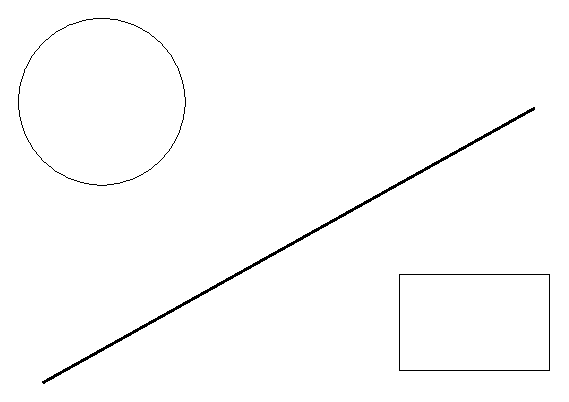
\includegraphics[width=0.5\columnwidth]{figures/fig.eps}
 \end{center}
 \caption{\label{figure:sample}図のタイトル}
\end{figure}

\subsection{そのまた次}

\section{最後}


